% paper/sections/casestudy3.tex — Case Study 3: FTS forecasting of PM10 air pollution.
% Revised in the pre-arXiv review pass; all numbers are printed by paper/code/casestudy3.py.

\subsection{Functional Time Series Forecasting: Daily PM10 Air Pollution}
\label{subsec:cs3-fts}

The Graz PM10 dataset~\citep{aue_norinho_hormann_2015} records the
concentration of airborne particulate matter (aerodynamic diameter
$<10\,\mu$m, in $\mu$g/m$^3$) at half-hourly resolution at the Graz-Mitte
station, from 2010-10-01 to 2011-03-31.  Reshaping the record into one curve
per day gives a genuine functional time series: 182 consecutive daily curves,
each a 48-point diurnal PM10 profile.  Unlike a cross-sectional collection, the
curves are ordered in real calendar time, so forecasting \emph{the next day's}
pollution profile is a substantive task~\citep{hyndman_ullah_2007,hormann_kokoszka_2010}.
Following \citet{aue_norinho_hormann_2015}, we model the data on the
variance-stabilising square-root scale and back-transform forecasts to
$\mu$g/m$^3$.

\paragraph{Model.}
\texttt{fdars.fts.ftsm(X, ARG, ncomp=3)} fits the functional principal
component decomposition of the curve sequence and an independent univariate
autoregressive model to each of the three score series (Yule--Walker
estimation, order chosen by AIC); \texttt{fdars.\allowbreak fts.\allowbreak
ftsm\_forecast} forecasts the scores and reconstructs the curves.
Figure~\ref{fig:cs3-curves} shows the 182 daily curves together with the FTS
mean, exposing the diurnal structure and the wide day-to-day amplitude
variation the model must capture.

\paragraph{Rolling-origin validation.}
A single train/test split is a fragile basis for judging a forecaster, so we
use a rolling origin.  For each of the last 30 possible forecast origins
(first forecast days 2011-02-24 to 2011-03-25) we fit the model on all days
before the origin and forecast seven days ahead.  Each forecast curve is
compared to the actual curve by root-mean-square error (RMSE, $\mu$g/m$^3$),
against two baselines: \emph{climatology} (the mean curve of the days before
the origin) and \emph{persistence} (the day before the origin).
At the one-day-ahead horizon the FTS forecast attains a mean RMSE of $17.69$,
against $26.18$ for climatology and $20.82$ for persistence; it beats
climatology at 26 and persistence at 20 of the 30 origins.  Averaged over all
seven horizons the mean RMSE is $21.32$ (FTS), $24.23$ (climatology), and
$27.02$ (persistence).  Figure~\ref{fig:cs3-forecast} shows the one-day-ahead
forecast at the final origin (left) and the mean RMSE at each horizon with
$\pm1$ standard-error bands (right).  The full analysis is reproduced by
\texttt{paper/code/casestudy3.py}.

\paragraph{Honest caveat.}
Forecast skill decays with horizon: the advantage over climatology is clear at
one day ahead but narrows to about one $\mu$g/m$^3$ at seven days, where a
low-rank curve model cannot anticipate day-specific pollution events.  The
study demonstrates that \texttt{fdars}' FTS interface produces skilful
next-day functional forecasts on a real temporal dataset; it is not a claim of
state-of-the-art air-quality forecasting.

\begin{figure}[tbp]
  \centering
  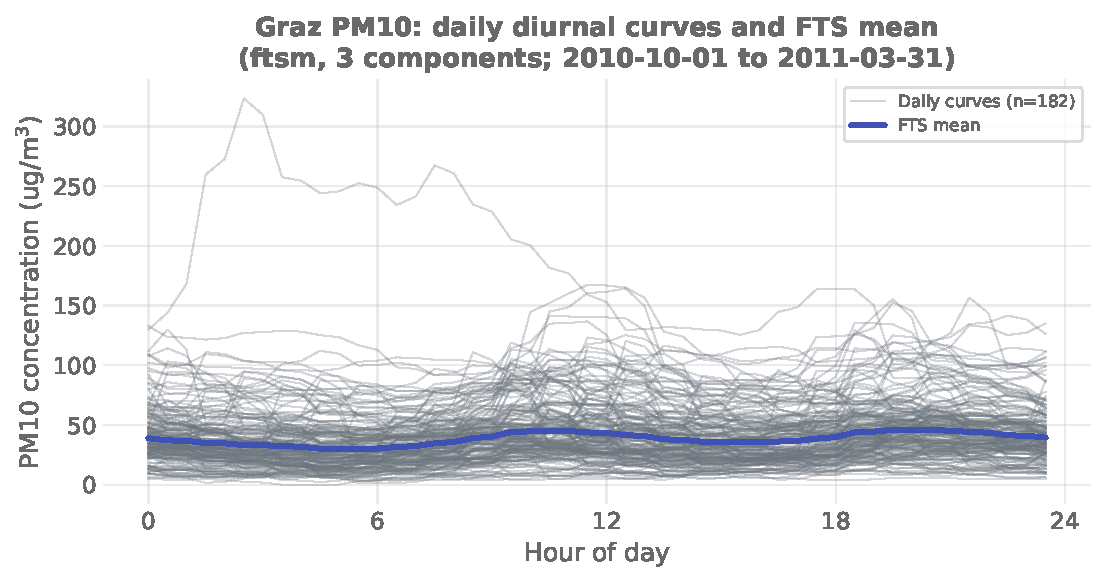
\includegraphics[width=\textwidth]{figures/cs3_pm10_curves.pdf}
  \caption{Graz PM10: the 182 daily diurnal curves (grey) and the FTS mean
    curve (solid, \texttt{ftsm}, 3 components).  Each day contributes one
    48-point functional observation; the $x$-axis is the hour of day.}
  \label{fig:cs3-curves}
\end{figure}

\begin{figure}[tbp]
  \centering
  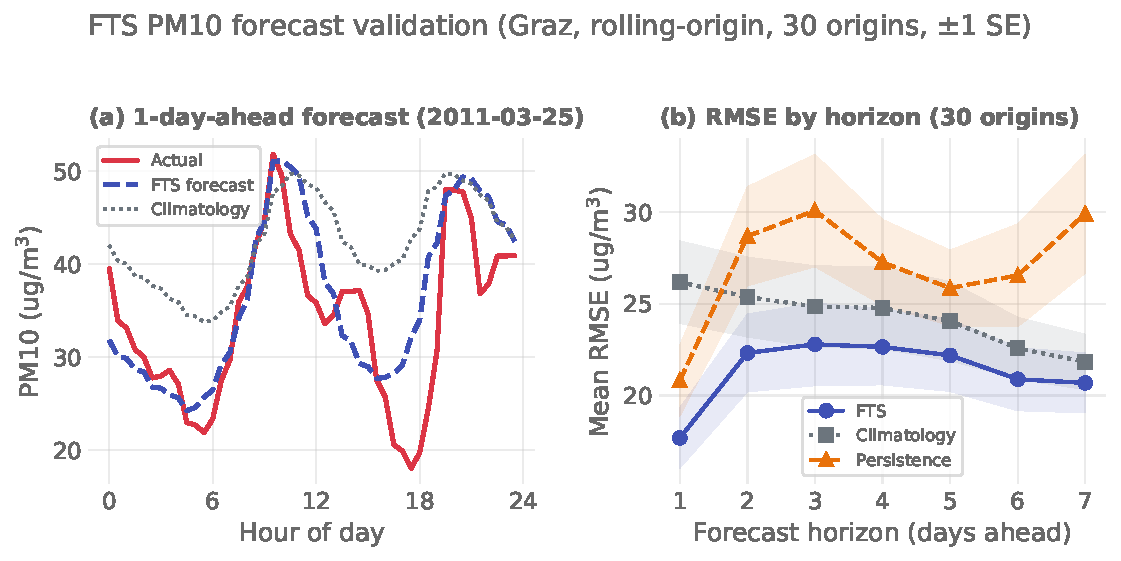
\includegraphics[width=\textwidth]{figures/cs3_pm10_forecast.pdf}
  \caption{Rolling-origin validation of the FTS PM10 forecast (30 origins).
    \emph{Left:} the one-day-ahead forecast at the final origin (2011-03-25)
    against the actual curve and the climatology baseline.  \emph{Right:} mean
    RMSE ($\mu$g/m$^3$) at each horizon for the FTS model, climatology, and
    persistence, with $\pm1$ standard-error bands.}
  \label{fig:cs3-forecast}
\end{figure}
